\chapter{Evaluation}
\label{evaluation}
Anschließend an die Implementierung der drei Funktionalitäten, welche das Aufzeichnen und Abspeichern von Tastatur-Eingabesequenzen, sowie das Senden von Tastatursignalen an das Betriebssystem von der SD-Karte und über Ethernet sind, folgt die Überprüfung und Evaluation eben dieser Funktionalitäten. Hierfür werden in den folgenden Teilabschnitten mögliche Tastatur-Eingabesequenzen verwendet, um die Implementierung sowohl mit Windows XP und Ubuntu 14.04 bei einem deutschen Tastaturlayout zu bestätigen. Ein Wechsel von einer Funktionalität zur anderen ist durch ein Umstecken des Drahtes zu den jeweiligen Pins der Funktionalitäten möglich.



\section{Aufnahme von Tastatureingaben}
Um die Korrektheit der Aufnahme und Abspeicherung von Tastatureingaben zu prüfen, wird zum einen beispielhaft der Titel dieser Bachelorarbeit über eine Tastatur eingegeben. Die Tastatur ist hierbei mit dem PS/2 Female Kabel der Implementierung verbunden und der PS/2 Male Anschluss mit einem PC. Die Eingaben werden wie erwartet in Form von Scancodes in der Textdatei auf der SD-Karte abgespeichert und gleichzeitig an den PC gesendet. Der Inhalt der Textdatei ist ein exakter Mitschnitt des zuvor eingegebenen Textes und in Abbildung \ref{reader} zu betrachten.
\begin{figure}
  \centering
  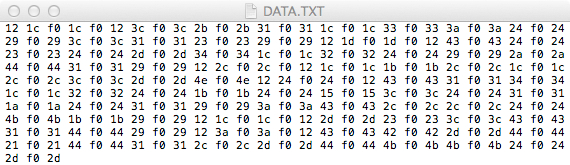
\includegraphics[width=1\textwidth]{images/reader.jpg}
  \caption{Bildschirmfoto der Textdatei nach Eingaben}
  \label{reader}
\end{figure}

\noindent Bei der Überprüfung anderer Tastatureingaben ist allerdings aufgefallen, dass die drei LEDs der Tastatur keine Rückmeldung erhalten haben. Falls also z.B. die Taste CAPS gedrückt wurde, registriert dies der PC zwar, jedoch wird das Signal für die LED nicht an die Tastatur weitergeleitet. Aufgrund einer fehlenden Fehlerbehandlung bei der Initialisierung der Tastatur, benötigt der Mikrocontroller eine angeschlossene Tastatur, sodass der Mikrocontroller nicht endlos auf eine Rückmeldung wartet. Bisher konnten auch keine USB-Tastatur mit PS/2-Adapter erfolgreich getestet werden.



\section{Wiedergabe von Tastatureingaben mittels SD-Karte}
Zur Überprüfung der zweiten Funktionalität werden Tastatureingaben in Form von Scancodes in die Textdatei auf der SD-Karte geschrieben. Diese Eingaben bewirken das Aufrufen einer Konsole und mithilfe eines Konsolenbefehls das Öffnen des Standardbrowsers mit der Startseite von Google. In Tabelle \ref{windows_test} sind diese für Windows XP einmal in Prosa und in Scancodes dargestellt. Der eigens eingeführte Scancode zur Verzögerung kommt an gegebenen Stellen auch zum Einsatz, um sicherzustellen, dass der PC die Tastatureingaben auch verarbeitet hat.
\begin{table}
  \begin{tabularx}{\textwidth}{|X|} \hline
    WINDOWS+R (wait) cmd (wait) ENTER (wait) start www.google.de (wait) ENTER \\ \hline
    e0 1f 2d f0 2d e0 f0 1f 00 00 00 21 f0 21 3a f0 3a 23 f0 23 00 00 00 5a f0 5a 00 00 00 1b f0 1b 2c f0 2c 1c f0 1c 2d f0 2d 2c f0 2c 29 f0 29 1d f0 1d 1d f0 1d 1d f0 1d 49 f0 49 34 f0 34 44 f0 44 44 f0 44 34 f0 34 4b f0 4b 24 f0 24 49 f0 49 23 f0 23 24 f0 24 29 f0 29 00 00 00 5a f0 5a \\ \hline
  \end{tabularx}
  \caption{Windows XP Tastatureingaben}
  \label{windows_test}
\end{table}

Wird nun der Mikrocontroller über das PS/2 Male Kabel an einen Windows PC angeschlossen, so werden diese Tastatureingaben einmalig ausgeführt. Das Ergebnis dieser Eingaben und der daraus folgende Browseraufruf sind in Abbildung \ref{writer} dargestellt.
\begin{figure}
  \centering
  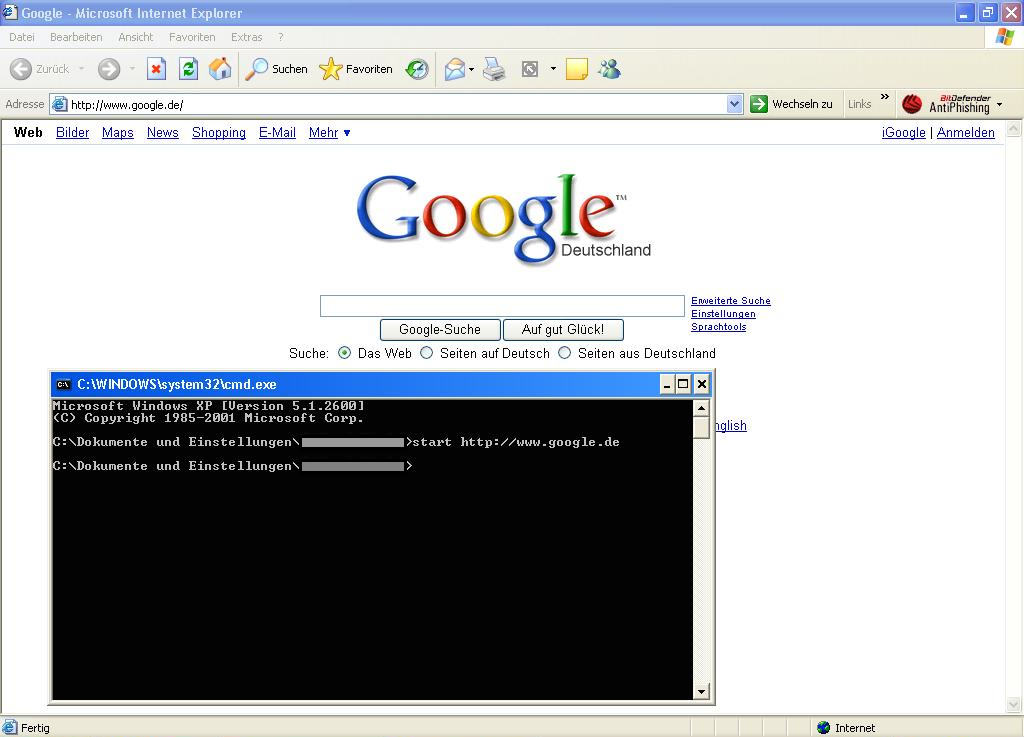
\includegraphics[width=1\textwidth]{images/writer.jpg}
  \caption{Bildschirmfoto der Wiedergabe auf Windows XP}
  \label{writer}
\end{figure}

Um ein entsprechendes Ergebnis unter Verwendung eines anderen Betriebssystems zu erhalten, z.B. Ubuntu 14.04, müssen die entsprechenden Tastatureingaben auch in Scancodes auf der SD-Karte hinterlegt werden. Tabelle \ref{linux_test} zeigt dies entsprechend mit der dazugehörigen Beschreibung.
\begin{table}
  \begin{tabularx}{\textwidth}{|X|} \hline
    CTRL+ALT+T (wait) xdg-open www.google.de (wait) ENTER \\ \hline
    14 11 2c f0 14 f0 11 f0 2c 00 00 00 22 f0 22 23 f0 23 34 f0 34 12 f0 12 4a f0 4a 44 f0 44 4d f0 4d 24 f0 24 31 f0 31 29 f0 29 1d f0 1d 1d f0 1d 1d f0 1d 49 f0 49 34 f0 34 44 f0 44 44 f0 44 34 f0 34 4b f0 4b 24 f0 24 49 f0 49 23 f0 23 24 f0 24 29 f0 29 00 00 00 5a f0 5a \\ \hline
  \end{tabularx}
  \caption{Ubuntu 14.04 Tastatureingaben}
  \label{linux_test}
\end{table}

\noindent Erwähnenswert ist im Rahmen der Evaluation, dass die Verzögerung nur schätzungsweise und nicht präzise festgelegt werden kann. Dementsprechend sind zuweilen mehrere Versuche notwendig, um die Eingaben korrekt ausführen zu können. Wichtig ist in dem Zusammenhang auch, dass der Fokus der Eingabe nicht durch einen Mausklick auf ein anderes Fenster gelenkt werden sollte, da sonst die Tastatureingabe ihren Zweck verfehlen könnte. Abgesehen von diesen Umständen ist eine automatisierte Wiedergabe von Tastatureingaben mithilfe des Mikrocontrollers und der SD-Karte möglich.



\section{Wiedergabe von Tastatureingaben über Ethernet}
Für die dritte Funktionalität, die Wiedergabe von Tastatureingaben über Ethernet, wurde ein weiteres mal der Titel dieser Bachelorarbeit als Eingabe verwendet. Um die Korrektheit dieser Funktionalität zu überprüfen wurde der Mikrocontroller via Ethernet an ein Netzwerk angeschlossen. Über einen anderen im Netzwerk verfügbaren PC kann dann die IP-Adresse im Browser eingegeben werden, sodass die Webseite des Mikrocontrollers angezeigt wird. In Abbildung \ref{website2} ist diese noch einmal mit den Scancodes des eingegeben Titels der Bachelorarbeit dargestellt.
\begin{figure}
  \centering
  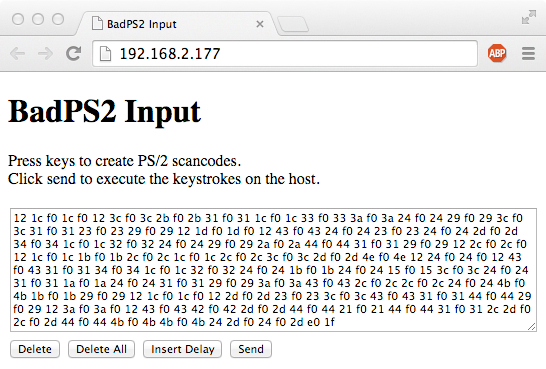
\includegraphics[width=1\textwidth]{images/website2.jpg}
  \caption{Bildschirmfoto der Webseite}
  \label{website2}
\end{figure}

Mit einem Klick auf ``Send'' werden die Scancodes an den Mikrocontroller und von dort aus direkt an den angeschlossenen PC abgesendet. Falls dort z.B. ein Texteditor geöffnet ist, erscheint dort dann der Titel dieser Bachelorarbeit.

\noindent In diesem Zusammenhang ist zu beachten, dass der Mikrocontroller nicht unbegrenzt große Tastatur-Eingabesequenzen entgegennehmen kann. Dies liegt einerseits an der Speichergröße des Mikrocontrollers, die 256 KB RAM beträgt. Andererseits liest der Mikrocontroller die Eingaben über die URL ein, da das Fomrular einen HTTP GET Request ausführt. Die Begrenzung der Zeichen in einer URL sind browserabhängig, liegen z.B. beim Internet Explorer bei 2083 Zeichen \cite{url_length}. Um dieses Problem zu beheben wäre die Verwendung einer Bibliothek notwendig, wie z.B. Webduino \cite{webduino}.